%%%%%%%%%%%%%%%%%%%%%%%%%%%%%%%%%%%%%%%%%%%%%%%%%%%%%%%%%%%%%%%%%%%%%
% LaTeX Template: Project Titlepage Modified (v 0.1) by rcx
%
% Original Source: http://www.howtotex.com
% Date: February 2014
% 
% This is a title page template which be used for articles & reports.
% 
% This is the modified version of the original Latex template from
% aforementioned website.
% 
%%%%%%%%%%%%%%%%%%%%%%%%%%%%%%%%%%%%%%%%%%%%%%%%%%%%%%%%%%%%%%%%%%%%%%

\documentclass[12pt]{report}
\usepackage[a4paper]{geometry}
\usepackage[myheadings]{fullpage}
\usepackage{fancyhdr}
\usepackage{lastpage}
\usepackage{graphicx, wrapfig, subcaption, setspace, booktabs}
\usepackage[T1]{fontenc}
\usepackage[font=small, labelfont=bf]{caption}
%\usepackage{fourier}
\usepackage[protrusion=true, expansion=true]{microtype}
\usepackage[english]{babel}
\usepackage{sectsty}
\usepackage[utf8]{inputenc}
\usepackage[authoryear, round]{natbib}
\bibliographystyle{abbrvnat}
\usepackage{url, lipsum}
\usepackage{mathptmx}
\usepackage{url}
\usepackage{amsmath}
\renewcommand\thesection{\arabic{section}}



\newcommand{\HRule}[1]{\rule{\linewidth}{#1}}
\onehalfspacing
\setcounter{tocdepth}{5}
\setcounter{secnumdepth}{5}

%-------------------------------------------------------------------------------
% HEADER & FOOTER
%-------------------------------------------------------------------------------
%-------------------------------------------------------------------------------
% TITLE PAGE
%-------------------------------------------------------------------------------

\begin{document}
	
	\title{ \normalsize \textsc{CSC2528 Term Paper}
		\\ [2.0cm]
		\HRule{0.5pt} \\
		\LARGE \textbf{\uppercase{Domain Adaptation in Natural Language Processing}}
		\HRule{2pt} \\ [0.5cm]
		\normalsize \today \vspace*{5\baselineskip}}
	
	\date{}
	
	\author{
		Krishnapriya Vishnubhotla \\ 
		Department of Computer Science \\
		University of Toronto 
		 }
	
	\maketitle
	\tableofcontents
	\newpage
	
	\begin{abstract}
		
		Statistical learning methods rely on having large amounts of training data, either labelled or unlabelled. Traditional supervised methods assume the training and test data come from the same underlying probability distribution, but this assumption rarely holds in real world scenarios. Transfer learning is the study of methods that allow us to transfer knowledge across different but related tasks, domains and distributions. It is an extensively studied topic in machine learning, and specifically for natural language processing. This work looks at the major approaches proposed for transfer learning tasks, how they've been adapted in the context of neural networks and deep learning, and compares their performance for a specific application: part-of-speech tagging. We'll also take a brief look at a few related tasks that have gained a lot of attention recently, such as multi-task learning and few-shot learning. 
		
	\end{abstract}

	
	\section{Introduction}
	Natural Language Processing (NLP) systems, when used out in the wild, often result in performance below what is expected or observed during experimental testing. This is because statistical classifiers assume that both the training and test data come from a common underlying distribution \citep{li2012literature}, but oftentimes the training data is too restricted/specialised to provide an accurate estimate of this. The problem relates to one of the core challenges in designing a computational language understanding system: natural language is highly variable and sparse \citep{goldberg2017neural}. The number of sentences that can be framed using the English language could never possibly be enumerated, and it therefore becomes extremely challenging to assemble a representative "training set for the English language". 
	\par
	Nevertheless, we can try. Generalizability of a statistical model is a highly desirable property, and much research has been done on preventing overfitting to the train set. The property of a model that allows it to draw conclusions on data it hasn't encountered before is called it's \textit{inductive bias} \citep{baxter2000model}. For example, the inductive bias of a linear regression model is that there exists a linear relationship between the input and the output. A rote learner, therefore, lacks any inductive bias. It is a term closely related to the above discussion on the distribution of data - \citep{torrey2010transfer} define inductive bias of a model as "the set of assumptions about the true distribution of the training data". Clearly, the better the inductive bias of a model, the better it's generalizability.
	\par
	Consider this: most part-of-speech tagging systems were trained on the Wall Street Journal (WSJ) corpus, containing news articles from the financial domain. A commonly cited example in literature is that of the word "monitor" \citep{li2012literature}. In the WSJ corpus, the word most probably is used as a verb, but in another domain, say Amazon electronic product reviews, it would be used as a noun. How would a PoS tagger know this, if it has only seen "monitor" as a verb? Intuitively, we expect the tagger to make decisions based on sentence structure and context words, and not just surface features. Thus, achieving a good inductive bias for NLP tasks implies a good understanding of syntax and semantics. This has been the focus of recent work on improving transferability of deep neural networks for NLP - obtaining generalizable, dense representations for words and sentences that work well across a range of tasks \citep{peters2018deep}. Unfortunately, this transferability hasn't moved beyond the first layer, and  we still need quite a bit of labelled data to achieve good performance on a particular task.
	\par Rather than aim for the lofty goal of building a general natural language understanding model, techniques have been studied that facilitate transfer of knowledge and parameters from a source domain (our training set) to a target domain (our test set). Formally, the study of methods that allow learning across domains, tasks and distributions is called transfer learning \citep{pan2010survey}. The key motivation is that one can transfer knowledge from a source domain for which we have annotated data, to a target domain where such data is scarce. Another way of looking at this is that the source data affects the inductive bias of the model in the target space. A related idea is multi-task learning \citep{collobert2008unified}, where one simultaneously optimises a model for several different, but related, objectives. Transfer learning, by contrast, aims to achieve a high performance only on the target task. Some other related techniques that apply to the low-data scenario include zero-shot/few-shot learning, data augmentation methods, and building task-independant architectures.
	\par A plethora of methods have been proposed for transfer learning in text applications. Many of these focus and evaluate on certain tasks: sentiment analysis \citep{blitzer2007biographies} \citep{glorot2011domain}, Named Entity Recognition (NER) \citep{lee2017transfer}, part-of-speech tagging (PoS) \citep{blitzer2006domain}, machine translation \citep{chu2017empirical} etc. The recent surge in neural methods for NLP has also led to a surge in corresponding transfer learning methods. Before we look at these, let us first formally define a few terms that will be used throughout the rest of the paper. 
	\subsection{Formal Definitions}
	We will use here the notation defined in \citep{pan2010survey} that is also followed in most transfer learning papers since.
	\begin{itemize}
		\item \textbf{Domain}: A domain $\textbf{D}$ has two components: a feature space $\chi$, and a marginal probability distribution $P(X)$. $P(X)$ here is the underlying distribution of our training data. The feature space varies based on how we define our features - for a binary bag-of-words representation of a text document, the feature space would be the set of all possible binary term vectors.
		\item \textbf{Task}: Given a domain $\textbf{D} = \{\chi, P(X)\}$, a task $T$ defines a label space $\gamma$ and a predictive function $f: \chi \rightarrow \gamma$. This predictive function is learnt from the data and constitutes our model. 
	\end{itemize}
	For a supervised learning task, we have a set of $n$ training examples, denoted by $D = \{(x_{i}, y_{i}) \in \chi \times \gamma: i \in (1,..,n)\}$. Our predictive function $f(.)$ is then equivalent to $P(y|x)$ for an $(x,y) \in D$. We will denote our source domain data and target domain data with $D_{s}$ and $D_{t}$ respectively. Similarly, the source and target tasks will be referred to by $T_{s}$ and $T_{t}$.
	\par With the above notations, we can refine our definition of transfer learning as techniques that utilise the knowledge in $D_{s}$ and $T_{s}$ to improve the learning of $T_{t}$ in $D_{t}$, where either $D_{t} \neq D_{s}$ or $T_{t} \neq T_{s}$. Note that, if both $D$ and $T$ are the same for the source and target domains, then it reduces to a general supervised learning problem.
	
	
	\subsection{Categories of Transfer Learning}
	Depending on the relationship between $D_{s},\, D_{t},\, T_{t}$ and $T_{s}$, we end up with slightly different scenarios of transfer learning, with a  different set of algorithms proposed for each:
	\begin{enumerate}
		\item \textbf{$\chi_{s} \neq \chi_{t}$} \\ This is the case when the feature spaces of our domains are different. In NLP, this commonly occurs when we're dealing with documents written in different languages (cross-lingual adaptation).
		\item \textbf{$P(X_{s}) \neq P(X_{T})$ }\\Here, the feature spaces are the same but the underlying data distributions are different. Our initial example of PoS tagging with the WSJ and bio-medical texts falls into this category, and is referred to as \textit{domain adaptation}. Thus, our source and target tasks are the same, but we're dealing with datasets from different domains. 
		\item $P(Y_{s}|X_{s}) \neq P(Y_{t}|X_{t})$ \\
		Both the source and target distributions share the same output labels, but the conditional distributions of these classes is different, i.e, the classes are unbalanced. Several class balancing techniques like SMOTE and random undersampling exist to deal with these, though they are far from perfect.
		\item $P(Y_{s}) \neq P(Y_{t})$ \\
		This case usually occurs alongisde case 3, where the supervised task itself is different for the source and target domains. Most of the recent research on neural transfer learning falls under this scenario. An application in NLP is where the source task involves binary classification, whereas the target task is a 10-way, perhaps more fine-grained, classification.
	\end{enumerate}
	The focus of this paper will be mostly constrained to case 2, domain adaptation (DA). Algorithms proposed for this fall under one of three categories: feature representation based \citep{daume2007frustratingly} \citep{collobert2008unified} \citep{blitzer2006domain}, instance  based \citep{xu2011instance} \citep{jiang2007instance} \citep{ruder2017learning} , and prior based \citep{chelba2006adaptation} \citep{finkel2009hierarchical}. In the context of neural NLP, we have work on learning general, off-the-shelf vector representations of words, such as word2vec \citep{mikolov2013distributed}. Language modelling is seen as a task that utilises most of the syntactic and semantic features of words, and is therefore used to achieve more informative representations \citep{devlin2018bert} \citep{peters2018deep}. More specifically for DA, autoencoders have emerged as a popular method for achieving domain invariant representations \citep{yu2016learning} \citep{chen2012marginalized}. 
	\par In the following sections, we will first look at popular DA algorithms proposed before the explosion of deep learning based NLP methods. We will  then look more closely at how domain adaptation functions in the context of neural network approaches to NLP. Due it's recent popularity, we'll also take a brief look at multi-task learning \citep{changpinyo2018multi} and few-shot learning in NLP \citep{srivastava2018zero}. In Section \ref{app}, we present performance numbers for popular DA algorithms proposed for part-of-speech (PoS) tagging, and Section \ref{conc} concludes the survey.
	
	\section{Domain Adaptation in NLP}
	\subsection{What do we mean by different domains?}
		In the previous section, we looked at formal definitions for a domain and task. Intuitively, in NLP applications, different domains means that our datasets are generated by different sources, i.e, written by different people, relating to different topics, or are in different languages. For example, two different people may use different adjectives to praise the same product, or the same person may use different adjectives to praise two different products. 
		
	\subsubsection{Multilingual corpora } 
	Adapting algorithms for multiple languages has been a longstanding focus in natural language processing. Much of the initial work was done in the context of Machine Translation (MT). The M1 model, the first of IBM’s statistical alignment models, is basically defined as a statistical bilingual dictionary that captures word correlation across languages \citep{pinto2009statistical}. This model was subsequently adapted for cross-lingual text classification, information retrieval and inference. It is a field that has achieved notable results in the last few years, with the development of cross-lingual embeddings that can be inferred even with no parallel data. 
	

	\subsection{Main Approaches}
	For a general supervised classification problem, let us assume $\chi$ to be our feature space and $\gamma$ to be our set of labels. We also have a set of training instances $\{(x_{i}, y_{i}) \in \chi \times \gamma: i \in (1,..,n)\}$, where $(x_{i}, y_{i})$ are drawn from the underlying probability distribution $p(x,y)$. We are trying to recover this unknown distribution so we can predict the label for unlabelled input instances. Discriminative models directly model the distribution $p(y|x)$. Assuming a fixed set of parameters $\theta$ for the model family, our aim now becomes finding the following:
	\[
		\theta^{*} = argmax_{\theta} \int_{\chi} \sum_{y \in \gamma} p(x,y) log p(y|x;\theta)dx 
	\]
	
	Since we do not know the true underlying probability $p(x,y)$, we estimate it using the training data. This observed, empirical probability distribution is denoted by $p_{s}(x,y)$. When our test data now comes from a different distribution $p_{t}(x,y)$, our estimation of the optimal parameters $\theta^{*}$ is no longer optimal. \\
	Using Bayes rule, one can factorize $p(x,y)$ as $p(x,y) = p(y|x)p(x)$ or as $p(x,y) = p(x|y)p(y)$. Domain adaptation methods can be broadly classififed into three categories based on which terms they modify in the above equations in order to bring $p_{s}(x,y)$ closer to $p_{t}(x,y)$. 
	\begin{itemize}
		\item \textbf{Prior-based methods} \\
		These methods place different priors over the parameters or the labels to make the estimated $p_{s}(y|x;\theta)$ closer to $p_{t}(y|x)$. A prior over the label space $p(y)$ is usually used in generative models such as the naive Bayes.
		
		\item \textbf{Feature Representation based methods} \\ These methods change the underlying feature representation space $\chi$ such that $p_{t}(y|x)$ is similar to $p_{s}(y|x)$. 
		\item \textbf{Instance-based methods} \\
		These set of methods revolve around selecting and/or weighting instances in the source domain that are similar to those in the target domain. Thus, they focus on the distribution $p(x)$, or selecting $x$ such that $p(y|x)$ is roughly the same in both the source and target domains. 
	\end{itemize} 

	The adaptation algorithms in all three categories also vary in terms of the amount of labelled target data they require, dependence on the underlying classification model, and computational complexity. These facets of the algorithms will become clearer as we look at them in individual detail in the following sections.

	\section{Prior-based methods}
	Let us now look at domain adaptation methods that work by placing priors over parameters $\theta$ of the model $p(y|x;\theta)$. Discriminative classifiers usually assume a gaussian prior with zero mean over the parameters. This prior acts as a regularizer for the model, preventing overfitting. A distribution over parameters can be used to control how features behave in the target and source domains - those that have a similar effect in both domains will share the same prior value, whereas they will be pushed apart for features that behave differently. These methods generally assume a small amount of labelled data in the target domain. 
	\begin{enumerate}
		\item \citep{chelba2006adaptation} proposed a prior-based adaptation method for the automatic capitalisation task. Their classifier was a Maximum Entropy Markov Model (MEMM), and involves training two models sequentially on the source and target data. First, the source model is trained with a zero-mean gaussian mean over the parameters. The target model parameters are then initialised with a gaussian prior centered at the corresponding value estimated by the source model. New features in the target data are initialised with a zero-mean prior as usual. The target model is then trained to maximise likelihood of data as usual. 
		\item \citep{finkel2009hierarchical} extended the above model to work with multiple source and target domains. Their algorithm utilises a hierarchical structure of priors, with a high-level one that is domain-independent, and a lower level of domain-specific priors. The evidence present in each domain for a feature influences the domain-specific prior, which in turn pushes the top-level prior to the same value. This top-level prior is the default value for all the domains. Thus, in every domain, for a particular feature, the prior value defaults to that of the top-level, and conversely, domain-level priors affect the value of the top-level priors. The hierachical structure of this algorithm results in a large number of parameters that need to be estimated, and the computational complexity is therefore quite high.
	\end{enumerate}

	\subsection{Prior over label space}
	\citep{chan2006estimating} took a different approach towards adapting classifiers for word sense disambiguation in different domains. The authors assume that $p(x|y)$ remains the same across both domains, but the prior probabilities of the labels $p(y)$ (here, word senses) differ. In other words, the occurrence proportions of different word senses will vary depending on the corpus in consideration. Assuming no labelled data in the target domain, the Expectation-Maximization (EM) algorithm is applied to estimate prior probabilities of the labels for both naive Bayes and logistic regression classifiers.
	\par
	Learning under the above assumption has also been studied in machine learning as the class imbalance problem. A popular solution is to re-sample instances from the soure data such that this re-sampled data has the same class distribution as the target dataset. 
	
	\subsection{Fine-tuning classifiers}  
	A popular supervised domain adaptation method, especially in computer vision, is fine-tuning of classifiers. Starting from support vector machines \citep{yang2007adapting} to deep convolutional neural networks \citep{sharif2014cnn}, both transfer learning and domain adaptation have been hugly succesful for vision aplications. A classifier is first trained on a related, auxiliary task that has lablled data, and it's parameters are fine-tuned from those values using labelled data from the target domain. Specifically in the context of neural networks, the use of pre-trained ResNet models \citep{he2016deep} has become pervasive in almost every application. A new classification layer is added on top of the pre-trained block, and, depending on the amount of labelled data available, the top-k layers of the network are trained \citep{yosinski2014transferable}.
	\par In recent months, a slew of methods have been proposed that aim to replicate the above methods for NLP applications. Universal Language Model for Fine-Tuning (ULMFiT) \citep{howard2018universal} and Transformer networks \citep{vaswani2017attention} have been shown to achieve state-of-the-art (SoTA) results on sentiment classification tasks without large labelled datasets. We'll take a closer look at these deep learning methods in the feature-representation section of this survey. 
	\section{Instance-based methods}
	\label{instance}
	Instance-weighting frameworks seek to bring either the distribution of the data $p(x)$ or the conditional label distributions $p(y|x)$ closer by giving greater importance to those instances that behave similarly in both domains. This approach has a straight-forward justification, explained below.\\
	Let's assume a loss function for our classifier, $l(x,y,\theta)$. Our parameter estimation is now as follows:
	\[
		\theta^{*} = argmin_{\theta} \sum_{(x,y) \in \chi \times \gamma} p_{s}(x,y) l(x,y, \theta) 
	\]
	In the target domain, we wish to find
	\[
		\theta^{*} = argmin_{\theta} \sum_{(x,y) \in \chi \times \gamma} p_{t}(x,y) l(x,y, \theta)
	\]
	But our training instances are sampled from the source domain. Therefore, we re-write the above equation as:
	
	\begin{align*}
	\theta^{*} &= argmin_{\theta} \sum_{(x,y) \in \chi \times \gamma} \frac{p_{t}(x,y)}{p_{s}(x,y)} p_{s}(x,y)l(x,y, \theta) \\
	&\simeq argmin_{\theta} \sum_{i=1}^{N} \frac{p_{t}(x_{i}^{s},y_{i}^{s})}{p_{s}(x_{i}^{s},y_{i}^{s})} p_{s}(x_{i}^{s},y_{i}^{s})l(x_{i}^{s},y_{i}^{s}, \theta)\\
	&= argmin_{\theta} \sum_{i=1}^{N} \frac{p_{t}(x_{i}^{s},y_{i}^{s})}{p_{s}(x_{i}^{s},y_{i}^{s})} l(x_{i}^{s},y_{i}^{s}, \theta)
	\end{align*}
		
	Thus, we weight each training instance in the source domain by the ratio $\frac{p_{t}(x_{i}^{s},y_{i}^{s})}{p_{s}(x_{i}^{s},y_{i}^{s})}$. However, with no labelled instances the target domain, the above ratio is hard to compute. Proposed approaches compute this by employing various heuristics to measure similarity between two data points. \\
	\begin{enumerate}
		\item \citep{jiang2007instance} analyse the domain adaptation problem by splitting it into two types:
		\begin{itemize}
			\item \textbf{Labelling Adaptation} : This is the case when $p(y|x)$ differs in the source and target domains.
			\item \textbf{Instance Adaptation} : This is the case when $p(y|x)$ is mostly similar in both domains, but $p(x)$ differs. 
		\end{itemize}
		They propose the \textit{instance pruning} approach for labelling adaptation, where one actively removes those instances from the source domain for which $p_{s}(y|x)$ is different from $p_{t}(y|x)$, and an \textit{instance weighting} aprroach for the latter case. They also propose a general weighting scheme that combines the above two approaches, and estimate the weights for each instance by a set of heuristics inspired from self-training and semi-supervised learning methods. However, these methods require some labelled data in the target domain. They evaluate their method on PoS tagging, Named Entity Recognition (NER), and spam classification in different domains.
		
		\item The problem of instance adaptation has been studied in machine learning under the term \textit{covariate shift}. Solutions mainly revolve around matching first or second-order statistics of the source and target datasets (density ratio estimation) \citep{bickel2009discriminative}. 
		\item Specifically for NLP, instance weighting methods were studied for Statistical Machine Translation (SMT). In \citep{axelrod2011domain}, the authors train a language model on the target domain data, and rate source domain data based on their perplexity scores on the language model.
		\item \citep{xia2013instance} assume that that the training data contains some samples that are drawn from, or are very close to, the target domain distribution. They apply a semi-supervised learning technique called PU learning to identify and weight these instances, and evaluate their approach on cross-domain sentiment classification.
	\end{enumerate}
	
	
	\section{Feature-based approaches} \label{feature_based}
	These methods attempt to find a feature-space $\chi$ that minimizes the different between $p_{t}(y,x)$ and $p_{s}(y,x)$. With the advent of deep learning methods in NLP, it has become the most popular approach towards building domain and task invariant representations. We'll begin this section with a look some of the earlier algorithms proposed in this area, and then switch our focus to advances in neural methods and a discussion of the current state-of-the-art.
	\begin{enumerate}
		\item \textbf{EasyAdapt} \\
		\citep{daume2007frustratingly} propose a "frustratingly easy" approach to supervised domain adaptation, where each original feature is replicated thrice - as a source-specific, target-specific and domain invariant version. Features that behave similarly across domains will have a large weight for the domian-invariant version, whereas domain-specific features will have a higher value in their specific domains. For example, going back to our part-of-speech tagging task for the WSJ dataset vs product reviews, consider two words: 'the' and 'monitor'. The feature 'the as a determiner' is common across domains, which means it's domain-specific weight is higher. The feature 'monitor as a verb' will have a large weight in the WSJ domain, and 'monitor as a noun' for the target domain. A common classifier is trained on samples from the source and target domain to obtain these weights. One evident disadvantage is that a substantial amount of labelled target data is needed to achieve a reliable estimate of these weights, though a semi-supervised improvement was suggested in a later paper titled EasyAdapt++ \citep{daume2010frustratingly}. 
		
		\item \textbf{Structural Correspondence Learning (SCL)} \\
		Proposed by \citep{blitzer2006domain}, SCL introduced the idea of using \textit{pivot features}, a concept that has been adopted by several other domain adaptation methods proposed since. Pivot features are those that behave similarly in both source and target domains, and are also indicative of the behaviour of non-pivot features. Thus, an important feature of the algorithm is that it can model hidden \textit{correlations} between features, rather than just dealing with lexical similarities. 
		\par Let us consider the following set of sentences (Figure \ref{Fig1}) from two corpora - the WSJ and the BIO corpus, which contains abstracts of publications in the medical domain. 
		\begin{figure}[h]
			\caption{}
			\label{Fig1}
			\centering
			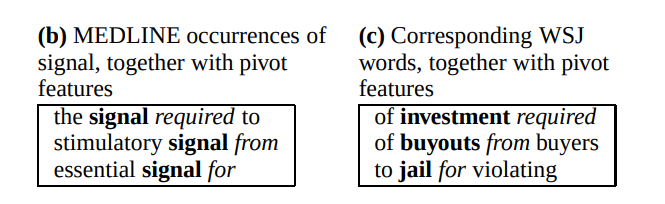
\includegraphics[width=0.7\textwidth]{pivot}
		\end{figure}
	
	   The words in italics are pivot features - they have the same part-of-speech tags in both domains. Further, they are indicative of the PoS tags of the non-pivot features, i.e, the words in bold. Thus, we can say that if "required" appears to the right of a word, then that word is likely to be a noun. \\
	   The SCL algorithm proceeds as follows:
	   \begin{enumerate}
	   	\item Define $m$ pivot features.
	   	\item Build $m$ linear classifiers for each of the pivot features to model the correspondence between them and the non-pivot features. Let the joint weight matrix of these classifiers be $W$.
	   	\item Obtain a projection matrix $\theta$ by performing Singular Value Decomposition (SVD) on $W$. 
	   	\item Project the original features $\chi$ into this new space, $\theta\chi$. 
	   	\item Train a classifier on the source domain using both the original and the transformed feaures.
	   \end{enumerate}
   
   SCL can be used both with and without labelled data in the target domain. The key idea is that if two non-pivot features from different domains are highly correlated with the same pivot features, then they will be projected to the same space in the latent space. Thus, our classifier trained with the transformed features on the source domain should also be effective in the target domain. 
   
		
		\item \textbf{Distributed representations} \\
		Distributed representations are currently the most pervasive and popular approach to task-invariant learning. Before jumping into neural models, we'll briefly look at some of the early work in building latent representations of words.
		\par Distributed representations refer to encodings of words as continuous vectors in some n-dimensional latent space. In contrast to symbolic, or one-hot, encodings, they allow us to capture notions of similarity among words - and also make them easier to use with statistical optimization techniques like gradient descent. 
		\par One of the earliest influential works in distributional semantics was Latent Semantic Analysis/Indexing (LSA/LSI) \citep{deerwester1990indexing}, a count-based method that used SVD to obtain latent representations. This was followed by other topic-model based methods such as Probabilistic LSA (PLSA) \citep{hofmann1999probabilistic} and Latent Dirichlet Allocation (LDA) \citep{blei2003latent}. In the context of domain adaptation, these techniques are used to identify common latent topics among different corpora, and a model is trained using only the common features \citep{guo2009domain}. Though the need for labelled target data is eliminated, topic models usually involve hyperparameters that are hard to set without some ground truth knowledge (such as the number of topics).
		
	\end{enumerate}
 	 The surveys in \citep{pan2010survey}, \citep{li2012literature} and \citep{jiang2008literature} provide an excellent and more detailed guide to the above mentioned methods. In the following section, we'll shift our focus to domain adaptation and transfer learning approaches involving neural architectures.
	\section{Domain Adaptation with Neural Networks}
	As mentioned before, transfer learning techniques with neural networks have seen great success in the computer vision domain. Pre-trained representations obtained from deep Convolutional Neural Networks (CNNs) trained for object recogntition on the ImageNet dataset \citep{deng2009imagenet} have worked extremely well across a wide array of tasks \citep{huh2016makes}. The various layers of the CNN model hierarchically capture different facets of an object - the lower layers capture features such as edges and contours, higher level layers capture more complex features like body parts and faces. For a new task, one can simply use these off-the-shelf representations along with a shallow network for classifiation, with fine-tuning if needed. 
	\par The success of the above method implies that object recognition, as a task, involves extracting knowledge that is relevant for several other vision tasks as well, such as image captioning. Unfortunately, we are yet to find such a generic proxy objective for language understanding. The closest we have come is perhaps language modelling - contextual representations obtained from networks trained on next word prediction tasks are just beginning to gain traction. Pretrained representations with fine-tuning fall under the supervised domain adaptation category, and the main aim of most of the following methods is to obtain representations that work well across a range of tasks and domains.
	
	\subsection{Pre-trained Representations}
	Neural representations were the successors to the distributed methods we looked at in section \ref{feature_based}. In \citep{bengio2003neural}, the authors first coined the term \textit{word embeddings} for continuous representations obtained via language modelling with multi-layered perceptron networks (MLP). They were further popularised by Collobert and Weston in 2008 \citep{collobert2008unified}. Their work combined word embedding training with several downstream tasks such as part-of-speech tagging and semantic role-labelling using convolutional networks. The general architecture of these models is shown in Figure \ref{fig_2}, taken from \citep{DSC:2016}.
	\begin{figure}[h] 
		\centering
		\caption{A Neural Language Model}
		\label{fig_2}
		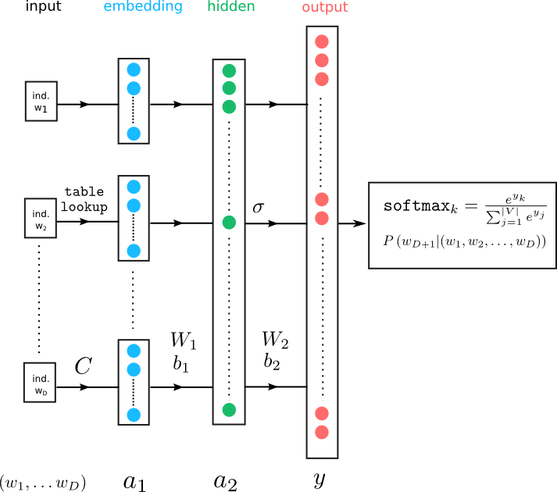
\includegraphics[]{nlm}
	\end{figure} 
	The hidden layer in the figure can be a single fully connected layer, an MLP, a deep CNN, a Recurrent Neural Network (RNN), and so on. Word representations are obtained from the blue embedding layer, which is usually randomly initialised and then trained along with the model parameters. The objective function can be any task. \citep{bengio2003neural} used language modelling, while \citep{collobert2008unified} trained their network jointly on six tasks and showed that multi-task learning leads to better representations. Their work shared only the embedding layer among different task architectures, but this need not always be the case.
	
	\subsection{word2vec and GloVe}
	The deep neural representations described above proved too computationally intensive to be widely adopted in their time. \citep{mikolov2013distributed} and \citep{pennington2014glove} introduced two new methods that considerably reduced the complexity by utilising shallow architectures with no hidden layers. \citep{mikolov2013distributed}'s word2vec model is trained using only the words within an n-sized window of a target word, and employs tricks such as negative sampling and sub-sampling to reduce computation time. Pre-trained word2vec embeddings remain the most popular word representations till date, usually employed as the initial embedding layer of a task-specific network. 
	\par \citep{pennington2014glove} use global co-occurance information rather than just the local context used by word2vec, and train a regression model that seeks to minimize the difference between the vector dot product of two words and the log of their co-occurence ratio. 
	\par Evaluated on both semantic and syntactic tasks, these vectors were shown to perform better than distributional semantic models like LSA. 
	
	\subsection{ELMo, BERT and Fine-tuning}
	After word2vec, several improvements to building better word embeddings were proposed by way of character-level, subword-level and word sense embeddings \citep{santos2014learning} \citep{bojanowski2017enriching} \citep{trask2015sense2vec}. There was also work on building phrase-level, sentence-level and document-level vector representations \citep{li2015hierarchical}, however, the transferability of these  to different domains and tasks is unclear. 
	\par In what has been hailed as "NLPs ImageNet moment" \citep{NLPImage:2018}, the last two years have seen a resurgance of pre-trained language model embeddings. With better frameworks and architectures such as Transformers and attention mechanisms, they are on the verge of replacing word2vec as the go-to choice for word representations. Works such as ULMFiT, Embeddings from Language Models (ELMo) \citep{peters2018deep} and most recently, Bideirectional Encoder Representations from Transformers (BERT) \citep{devlin2018bert} show that language model pre-training on deep neural networks followed by fine-tuning of the top few layers gives state-of-the-art results on a wide range of NLP tasks like text classification, sequence tagging and natural language inference with only a few hundred samples -  a huge improvement over few thousand per-class samples usually needed.
	
	\subsection{Domain-specific embeddings}
	All of the above work focussed on supervised domain adaptation with general-purpose word representations. \citep{bollegala2015unsupervised} introduce the cross-domain word representation task, where the goal is to learn a domain-specific representation for each common word $w$. Inspired by the concept of pivot and non-pivot features introduced in \citep{blitzer2006domain}, they constrain the representations of pivot features to be similar across domains. Their objective function closely follows that of word2vec, but is limited to predicting non-pivot features from the surrounding pivot fetures. Evaluated on cross-domain sentiment classification, they showed that their method outperformed SCL and other baselines. 
	\par \citep{yang2017simple} alternatively add a regularisation term to  the word2vec objective, that measures the relevance of a word to each domain via a frequency-based similarity measure. It loosely follows the same inuition as \citep{bollegala2015unsupervised}, wherein they try to keep the vectors of words that are frequent in both domains as close to each other as possible. 
    \par Both of the above methods train a logistic regression classifier on the source domain dataset with the learned embeddings, and evaluate on the target domain. Thus, their only target domain requirements are a relatively large unlabelled dataset.
	
	\subsection{Autoencoder based domain adaptation}
	Autoencoders are another key representation learning approach, apart from the methods mentioned in the above sections. Autoencoders are networks that are trained to reconstruct the input representation. Mathematically, they comprise two functions: and enocder function $h(.)$ and a decoder function $g(.)$. The reconstruction is given by $r(x) = g(h(x))$, and the reconstruction error by some loss function $l(x,r(x))$. \citep{vincent2008extracting} proposed the stacked denoising autoencoder (SDA), where several autoencoders were sequentially stacked on top of one another, with the encoded output of the first serving as the input for the second and so on. The parameters of each level serve as hierarchical representations of the input, much like other deep neural networks. A denoising autoencoder, as opposed to the regular autoencoder, is fed a slightly corrupted input representation $\tilde{x}$ instead of $x$.
	\begin{enumerate}
		\item \citep{glorot2011domain} propose an SDA-based domain adaptation method for sentiment analysis. The SDA is trained on the unlabelled data from all domains to build effective feature representations, and an SVM classifier is then learnt on the source domain data. 
		\item  \citep{chen2012marginalized} improved the computational complexity of the above approach by proposing the marginalised SDA (mSDA) model, which allows only linear transformations in the denoisers. Their method achieved performance comparable to that of \citep{glorot2011domain}, while massively improving on the training time. 
	\end{enumerate}
	  
	\subsection{Domain-adversarial training}
	Another representation learning approach that achieved state-of-the-art sentiment classification results is domain-adversarial training \citep{ganin2016domain}. Like most of the above methods, it is based on the idea of learning \textit{domain-invariant representations}, rather than domain-specific ones. The authors introduce an additional loss term based on the model's prediction of which domain the input sample comes from. The model now tries to maximise this loss term, which effectively means that the representations of samples from different domains become indistinguishable. 
	
	\section{Related Work}
	In this section, we'll look at some concepts that are closely related to those of transfer learning, but either have enough work done in them to merit a separate field name, or do not fall under any specific methodological category.  
	\subsection{Looking at data}
	 Looking back at Section \ref{instance}, we see that instance weighting is a supervised domain adaptation algorithm. In \citep{plank2014importance}, the authors apply the technique to unsupervised cross-domain part-of-speech tagging and present a \textit{negative} result. After experimenting with different weighting schemes across six corpora, they conclude that most of the performance drop across domains is due to out-of-vocabulary words - an issue that importance weighting doesn't help much with. 
	 \par In \citep{plank2016non}, Prof. Barbara Plank takes a step back to ask what actually constitutes a domain difference, and discusses how models need to be able to detect this change and adapt to it without any prior knowledge of the target domain. For example, even within a single dataset such as social media tweets, one observes great variety in the language style relating to different social groups, topics, user demographics, etc. She introduces the term \textit{fortuitous data} for data that can be harvested from side-sources, such as Wiktionary, to help with unsupervised domain adaptation. Further work by her and others focusses on optimally selecting data for transfer learning purposes. \citep{ruder2017learning} uses Bayesian Optimisation to learn a measure of similarity between domains, and then find the most promising examples from the source domain for transfer. Looking at data and understanding when and why different transfer learning methods work (or do not work) is an important research direction, and one that can help us avoid \textit{negative transfer}. Negative transfer is when a transfer method actually decreases performance when compared to traditional supervised leaerning \citep{torrey2010transfer}.

	\subsection{Multi-task learning}
	Multi-task learning \citep{caruna1993multitask} seeks to optimise the objectives for several tasks simultaneously, as opposed to transfer learning that is concerned only with the target domain/task. Though the assumption is implicit that one has labelled data for every task, it's been observed that multi-task learning can push up the performance on a task with very little labelled data by leveraging information learnt from the other tasks. With neural networks, parameter sharing has emerged as a widely used multi-task learning technique where all network layers except the last classification one are shared among all tasks. We looked at one instance of this in NLP already, with the work in \citep{collobert2008unified} that used it to learn word representations. Recent work has leveraged it for cross-domain classification \citep{yu2016learning} \citep{liu2015representation}, representation learning \citep{hashimoto2016joint} and sequence tagging \citep{sogaard2016deep} \citep{rei2017semi}.
	
	\subsection{Few-shot learning}
	Few-shot learning, and other techniques like one-shot and zero-shot learning, refer to learning classifiers with very few (or zero, or one) example per class. It is motivated by the ability of humans to generalise and quickly learn new concepts with very little supervision; for example, learning to identify different animals. \citep{vinyals2016matching} explored this idea by focussing on two goals - rapid acquisition of new examples while providing excellent generalisation from common examples. Using neural networks that are augmented with memory space, they achieve an accuracy of around 40\% on a language modelling related task (predicting the missing word in a sentence). While not impressive compared to state-of-the-art methods, it is considerably above the random baseline of 20\%. Few-shot learning has been mostly succesful in cross-lingual learning in NLP  \citep{artetxe2018massively} \citep{upadhyay2018almost}.
	
	\subsection{Cross-lingual learning}
	
	Learning cross-lingual representations with minimal data has seen impressive improvements in recent times. Moving from bilingual to multilingual analysis, recent work has aligned word embeddings of more than 80 languages in a single latent space \citep{conneau2017word}. This allows us to translate between any two language pairs, even those with no parallel data between them, i.e., zero-shot translation. Cross-lingual embeddings also allow us to exploit similarities between languages that share typological properties, such as morphology and sentence structure \citep{johnson2017google}. 
	
	\subsection{Semi-supervised learning}
	If one ignores the domain difference between source and target datasets, the domain adaptation problem is very similar to that of semi-supervised learning. Semi-supervised learning methods typically assume limited availability of labelled data, and aim to make use of unlabelled data during training. Classic semi-supervised learning technqiues include self-training \citep{yarowsky1995unsupervised}, co-training \citep{blum1998combining} and boosting \citep{mallapragada2009semiboost}. \par
	\citep{ruder2018strong} considers how semi-supervised algorithms can be adapted to learn under domain shift. Their evaluation on sentiment classification and PoS tagging showed that these techniques achieved performance comparable to many neural and state-of-the-art transfer learning methods.
	
	
	
	\section{Case Study: Part-of-Speech tagging}
	\label{app}
	
	In this section, we look at one specific NLP application, part-of-speech tagging, and how the different domain adaptation methods we've talked above in previous sections fare on the task.
	\subsection{Why domain adaptation?}
	We briefly spoke about why domain matters in PoS tagging in the introductory section of this paper, with the word 'monitor' being used as a verb and a noun depending on the domain. Out-of-vocabulary (OOV) words provide another challenge, especially with new proper nouns being introduced in each domain. One can also imagine that domains like Twitter have very different sentence structures when compared to news articles.
	
	\subsection{Datasets}
	The standard dataset in English for tagging and parsing experiments is the Wall Street Journal (WSJ) portion of the Penn Treebank corpus \citep{marcus1993building}. The Syntactic Analysis of Non-Canonical Language (SANCL) 2012 shared task \citep{petrov2012overview} provided five more domains - newsgroups, weblogs, reviews, answers and emails.
	
	\subsection{Methods}
	We present numbers, where available, for the above datasets and the following methods:
	\begin{enumerate}
		\item SCL - Structural Correspondence Learning from \citep{blitzer2006domain}
		\item Stanford Tagger - A Maximum Entropy Markov Model used by the Stanford PoS tagger, \citep{toutanova2000enriching}.
		\item mSDA - The marginalised Stacked Denoisig Autoencoder from \citep{chen2012marginalized}.
		\item FLORS - A representation learning based model proposed specifically for PoS tagging that uses handcrafted features like word suffixes, \citep{schnabel2014flors}.
		\item FEMA - Feature EMbeddings for domain Adaptation, a representation learning model proposed specifically for PoS tagging that used feature embeddings along with domain attribute embeddings, \citep{yang2015unsupervised}.
		\item Bi-LSTM - A bidirectional Long Short Term Memory network (LSTM) based tagger from \citep{plank2016multilingual}.
	\end{enumerate}
	

	
	\subsection{Results}
	\label{pos_res}
	
	Table \ref{pos_results} below lists the F1 scores obtained by each of the above methods. The numbers on the source domain test set, i.e, WSJ, average around 97\% for all the methods, and is the accepted SoTA. However, performance on the other domains is at least 5-6\% percentage points lower. This difference is also dependent on the target domain itself - the EMAILS domain consistently proves to be the hardest to adapt to. This further drives home the importance of looking at data and being able to adapt dynamically to the domain.
	
	\begin{table}[h]
		\caption{$F_{1}$ scores of DA algorithms for PoS Tagging. Best results in each domain are highlighted in bold.}
		\label{pos_results}
		\begin{tabular}{|l|l|l|l|l|l|l|l|}
			\hline
			& WSJ   & ANSWERS & NEWSGROUPS & WEBLOGS & EMAILS & REVIEWS \\
			\hline
			SCL             & -     & 90.04   & 91.51      & 92.32   & 88.04  & 90.29   \\
			\hline
			Stanford Tagger & 97.43  & 89.74   & 91.25      & 92.32   & 87.77  & 90.30   \\
			\hline
			Bi-LSTM         & \textbf{97.50}   & 90.43   & 91.83      & 92.44   & 87.95  & 90.04   \\
			\hline
			mSDA            & -       & 90.61   & 91.83      & 92.39   & 88.11  & 90.95   \\
			\hline
			FLORS           & 97.11  & 91.17   & 92.41      & 93.14   & 88.67  & \textbf{92.25}   \\
			\hline
			FEMA            & -       & \textbf{91.35}   & \textbf{92.60}      & \textbf{93.43}   & \textbf{89.02}  & 92.15  \\
			\hline
		\end{tabular}
	\end{table} 
	
	\subsection{Discussion}
	One problem while evaluating performance of an algorithm across domains is inconsistencies in tag annotation. In \citep{schnabel2014flors}, the authors draw attention to some examples of this: file names, such as "xyz.doc" are annotated as NN, whereas their behaviour is closer to that of NNPs. For the BIO dataset introduced in \citep{blitzer2006domain}, many bio-specific names are again annotated as NNs rather than NNPs. They show that converting all NNP tags to NN improved the $F_{1}$ scores of algorithms by almost 4 percentage points. 
	\par Further anaysis by them and in \citep{ruder2018strong} examines how algorithms fare on OOV words, unknown tags and unknown word-tag combinations. FLORS, which uses contextual information, performs much better on these categories than other methods that use lexical information, as is to be expected. An important point mentioned is that there are some things DA simply cannot do, such as predicting tags that don't occur anywhere in the training data.
	\par Finally, the top two systems from Table \ref{pos_results} are both designed specifically for the task at hand. General purpose embeddings like word2vec are far from reaching SoTA on unsupervised domain adaptation. This is also the case for other NLP applications like named entity recognition and sentiment analysis, and indicates that we are far from finding optimal representations that are pertinent to multiple tasks simultaneously.
	
	
	\section{Conclusion}
	\label{conc}
	In this survey, we have attempted to provide a brief overview of domain adaptation methods for natural language processing. We have covered the broad categories under which DA algorithms fall and their mathematical underpinning, however, it is by no means comprehensive with regards to papers that have been published under the topic. \par Many domain adaptation methods have been formulated specifically for certain applications. Sentiment analysis in particular has seen a lot of work in the area. Recently, there has been an increased focus on analysing social media data, especially that of Twitter, with algorithms desgined to deal with its format of short text, hashtags and emoticons. For sequence labelling tasks like Named Entity Recognition (NER) and PoS tagging, heterogenous label sets and OOV words present a significant challenge. 
	\par With recent efforts concentrating on building domain and task invariant word representations, the line between domain adaptation and transfer learning has blurred. Deep neural models like ELMo can dynamically generate embeddings for a word based on the context it appears in, replacing word2vec as the de-facto choice for pre-trained word vectors. Large scale language-model pre-training followed by fine tuning has drastically reduced the labelled data requirements for classification tasks, though the number is still in the few thousands. Transfer learning is currently the field that is seeing the most interest and development in NLP.
	\par However, the performance numbers in Section \ref{pos_res} demonstrate that there is still a lot of progress to be made. Apart from building general purpose representations, one needs to explicitly identify and use target-domain specific data where necessary. Semi-supervised learning methods are seeing a resurgence in this regard, e.g., \citep{clark2018semi}. Cross-lingual learning is another relevant field that is receiving attention, and in particular, improving translation performance on low-resource languages.
	\par Shared tasks such as CLEF (\url{http://clef2018.clef-initiative.eu/index.php?}) and SemEval (\url{http://alt.qcri.org/semeval2019/index.php?id=tasks}) have been crucial in providing datasets and challenges encouraging development in these areas, and are also a good starting point to survey previous work. Other resources that I have found useful include NLP blogs (\url{http://ruder.io/}), libraries (\url{http://nlp.fast.ai/}) and last but not least, \#NLProc Twitter threads (\url{https://twitter.com/arxiv_cscl}).
	
	
	%-------------------------------------------------------------------------------
	% REFERENCES
	%-------------------------------------------------------------------------------
	\newpage
	
	\bibliography{references}
	
	
\end{document}

%-------------------------------------------------------------------------------
% SNIPPETS
%-------------------------------------------------------------------------------

%\begin{figure}[!ht]
%	\centering
%	\includegraphics[width=0.8\textwidth]{file_name}
%	\caption{}
%	\centering
%	\label{label:file_name}
%\end{figure}

%\begin{figure}[!ht]
%	\centering
%	\includegraphics[width=0.8\textwidth]{graph}
%	\caption{Blood pressure ranges and associated level of hypertension (American Heart Association, 2013).}
%	\centering
%	\label{label:graph}
%\end{figure}

%\begin{wrapfigure}{r}{0.30\textwidth}
%	\vspace{-40pt}
%	\begin{center}
%		\includegraphics[width=0.29\textwidth]{file_name}
%	\end{center}
%	\vspace{-20pt}
%	\caption{}
%	\label{label:file_name}
%\end{wrapfigure}

%\begin{wrapfigure}{r}{0.45\textwidth}
%	\begin{center}
%		\includegraphics[width=0.29\textwidth]{manometer}
%	\end{center}
%	\caption{Aneroid sphygmomanometer with stethoscope (Medicalexpo, 2012).}
%	\label{label:manometer}
%\end{wrapfigure}

%\begin{table}[!ht]\footnotesize
%	\centering
%	\begin{tabular}{cccccc}
%	\toprule
%	\multicolumn{2}{c} {Pearson's correlation test} & \multicolumn{4}{c} {Independent t-test} \\
%	\midrule	
%	\multicolumn{2}{c} {Gender} & \multicolumn{2}{c} {Activity level} & \multicolumn{2}{c} {Gender} \\
%	\midrule
%	Males & Females & 1st level & 6th level & Males & Females \\
%	\midrule
%	\multicolumn{2}{c} {BMI vs. SP} & \multicolumn{2}{c} {Systolic pressure} & \multicolumn{2}{c} {Systolic Pressure} \\
%	\multicolumn{2}{c} {BMI vs. DP} & \multicolumn{2}{c} {Diastolic pressure} & \multicolumn{2}{c} {Diastolic pressure} \\
%	\multicolumn{2}{c} {BMI vs. MAP} & \multicolumn{2}{c} {MAP} & \multicolumn{2}{c} {MAP} \\
%	\multicolumn{2}{c} {W:H ratio vs. SP} & \multicolumn{2}{c} {BMI} & \multicolumn{2}{c} {BMI} \\
%	\multicolumn{2}{c} {W:H ratio vs. DP} & \multicolumn{2}{c} {W:H ratio} & \multicolumn{2}{c} {W:H ratio} \\
%	\multicolumn{2}{c} {W:H ratio vs. MAP} & \multicolumn{2}{c} {\% Body fat} & \multicolumn{2}{c} {\% Body fat} \\
%	\multicolumn{2}{c} {} & \multicolumn{2}{c} {Height} & \multicolumn{2}{c} {Height} \\
%	\multicolumn{2}{c} {} & \multicolumn{2}{c} {Weight} & \multicolumn{2}{c} {Weight} \\
%	\multicolumn{2}{c} {} & \multicolumn{2}{c} {Heart rate} & \multicolumn{2}{c} {Heart rate} \\
%	\bottomrule
%	\end{tabular}
%	\caption{Parameters that were analysed and related statistical test performed for current study. BMI - body mass index; SP - systolic pressure; DP - diastolic pressure; MAP - mean arterial pressure; W:H ratio - waist to hip ratio.}
%	\label{label:tests}
%\end{table}